\chapter{Software Implementierung}

\section{PX4} \label{px4:subsection}
PX 4 ist eine Open-Source-Software, welche zur Steuerung verschiedener Arten von Fahrzeugen genutzt werden kann, hierzu zählen beispielsweise verschiedene Drohnenarten, sowie auch Fahrzeuge auf dem Boden und Unterwasserfahrzeuge.\\ Es kann zum einen für bereits flugfähigen Drohen eingesetzt werden. Aber es besteht auch die Möglichkeit eine neue Drohne in Verbindung mit PX4 zu bauen.\\
Für die Verwendung der PX4 Software kann QGroundControl (siehe Kapitel \ref{qGroundControl:subsection}) verwendet werden. \cite[vgl.][]{px4} \\
Der PX4-Flugstack wurde ursprünglich nur dür die Pixhawk-Hardware entwickelt, allerdings ist es heutzutage auch möglich diesen auf Linux-Computern und anderen Hardware einzusetzen. Wie es auch bei der Coex Clover Drohne mit dem Coex Pix umgesetzt wird. \\
Die Software setzt Sensoren, ein um den Zustand der Drohne zu bestimmen. Hierfür werden einige Sensoren vorausgesetzt, zu diesen zählen ein Gyroskop, ein Beschleunigungssensor, ein Magnetometer sowie ein Barometer. Zudem ist GPS empfohlen um weitere Modi nutzen zu können. \cite[vgl.][]{px4}

\subsection{Flugmodi}
PX4 bietet verschiedene Flugmodi an, welche das Verhalten der des jeweiligen Fahrzeuge beziehungsweise Drohnen steuert und auch regelt, wie jeweils auf Benutzereingaben regiert werden soll. Das Wechseln dieser Flugmodi kann zum einen über die QGroundControl Software (siehe Kapitel \ref{qGroundControl:subsection}) oder auch je nach Anpassung der Fernbedinung, beispielsweise über verschiedene Schalter, auf dieser vollzogen werden. \\
Allerdings muss auch beachtet werden, dass nicht alle Flugmodi bei allen Drohnen oder Fahrzeugen einsetzbar sind. Aussschlaggebend hierfür ist vor allem die Ausstattung des. Da jeder Flugmodi bestimmte Bedingungen hat die erfüllt sein müssen, beispielsweise Sensoren wie ein Geschwindikgeitssensor. \\
Die Flugmodi lassen sich in drei Kategorien einteilen, diese sind manuelle, ünterstütze sowie automatische Steuerung.
Da es bei diesem Projekt um den Einsatz einer Drohne handelt, werden im folgenden lediglich die für Drohnen relevanten Flugmodi erläutert.
Zu der manuellen Steuerung, bei welchem der Pilot die Drohne direkt und ohne direkte UNterstützung steuert, gehören unter anderem die Modi "manuell" beziehungsweise "stabilisiert". Diese sorgen für eine stabilisierte horizontale Ausrichtung, jedoch ermöglichen sie es dem Piloten hierbei, das Gaspedal sowie die Roll- und Neigbewegungen selbst zu bestimmen. Zu dieser Katergorie gibt es noch weitere Modi, welche allerdingsa hauptsächlich für Flugshows genutzt werden.
Bei der unterstützen Steuerung kann aus zwei verschiedenen Flugmodi gewählt werden, "ALTCTL (Altitude)" und "POSCTL (Position)". Beim ALTCTL-Modi wird besonders die Höhe der Drohne von Autopliot gesteurt, sodass diese einen möglichst konstanten Abstand zum Boden hält. Dieser Modi benötigt hierfür ein Barometer oder andere Sensoren zur Höhenmessung.
Der POSCTL dient zum Halten der Position der Drohne, das heißt neben der Höhe werden zudem die Bewegungsgeschwindkeit nach vorne, hinten und zur Seite gesteuert, um die Drohne möglichst auf einer bestimmten Position zu halten.\\
Bei der automatischen Steuerung fliegt die Drohne automatische ohne Benutzereingaben mittels eines Programms. Zu dieser Katergorie gehört der "Offboard"-Modus hierdurch ist es möglich, dass die Drohne durch einen anderen Computer gesteuert werden kann. Zudem gibt es noch einen Missions-Modus, hierbei kann beispielsweise über QGroundControl ein Pfad geplant werden, welcher dann von der Drohne mittels GPS geflogen wird. \\
Für das Projekt ist hierbei vor allem der Offboard-Modus von Bedeutung, da dieser benötigt wird, um autonome Flüge mit der Coex Clover Drohne zu machen, da diese hierbei von dem Raspberry Pi gesteuert wird. \cite[vgl.][]{flight-modes}


\subsection{QGroundControl}  \label{qGroundControl:subsection}
QGroundControl ist eine Software, welche vor allem für Drohnen mit einem PX4 aber auch anderen Flight Controller genutzt werden kann. Hierbei bietet es verschiedene Funktionen. Zum einen gehört hierzu die Konfiguration der einzelnen  Drohnen. Desweiteren ist es möglich mit der Software verschiedene Flugmodi auszuwählen, sowie diese dann auch während des Fluges zu überwachen, beispielweise durch die Anzeige der Flugposition auf einer Karte sowie auch deren Geschwindigkeit und andere Sensordaten.
Es ist auch möglich mit QGroundControl eine ganze Flugplanung zu machen, welche die Drohne daraufhin umsetzt. \cite[vgl.][]{qGroundControl}


\section{Systemarchitektur}

\subsection{Allgemeine Systemarchitektur eines ROS Programms}
Das Robot Operating System hat den Bereich der Robotik revolutioniert, indem es einen robusten und flexiblen Rahmen für die Entwicklung komplexer Robotersysteme bietet. Das Herzstück von \ac{ROS} ist seine ausgeklügelte Systemarchitektur, die das Zusammenspiel zwischen verschiedenen Komponenten orchestriert und eine nahtlose Kommunikation und Koordination ermöglicht.

\subsubsection{Zentrale Konzepte}
\begin{description}
    \item[Nodes:] Nodes sind autonome Softwaremodule, die bestimmte Aufgaben innerhalb eines ROS-Systems übernehmen. Sie kommunizieren miteinander, indem sie Nachrichten zu Themen veröffentlichen und abonnieren oder indem sie Services aufrufen und bereitstellen. Nodes können über mehrere Maschinen verteilt sein und bilden so ein verteiltes System. (Siehe Kapitel \ref{nodes:subsection})
    
    \item[Topics:] Topics sind benannte Busse, über die Nodes Nachrichten austauschen. Nachrichten werden von einem oder mehreren Nodes in Topics veröffentlicht und von Nodes abonniert, die am Empfang der Daten interessiert sind. Topics verwenden ein Publish-Subscribe-Messaging-Muster, das eine asynchrone Kommunikation ermöglicht und die Sender- und Empfängernodes entkoppelt. (Siehe Kapitel \ref{topics:subsection})
    
    \item[Messages:] Nachrichten sind die Datenstrukturen, die für die Kommunikation zwischen Nodes verwendet werden. Sie werden in ROS mithilfe der Interface-Definition Language (IDL) oder Nachrichtenbeschreibungsdateien (.msg) definiert. Nachrichten können einfach sein, z. B. numerische Werte oder Zeichenketten, oder komplex, bestehend aus verschachtelten Strukturen und Arrays. (Siehe Kapitel \ref{messages:subsection})
    
    \item[Services:] Services ermöglichen eine synchrone Anfrage-Antwort-Kommunikation zwischen Nodes. Ein Node bietet einen Service an, und andere Node können Anfragen an ihn senden. Die Dienstnode verarbeitet dann die Anforderung und sendet eine Antwort an den anfordernden Node zurück. Services werden mithilfe von .srv-Dateien definiert und folgen einem Client-Server-Kommunikationsmuster.
\end{description}

\subsubsection{Ebenen der ROS-Systemarchitektur}
\begin{description}
    \item[Dateisystem-Ebene:] Die Dateisystem-Ebene in \ac{ROS} spielt eine entscheidende Rolle bei der Organisation und Verwaltung der für die Entwicklung von Roboteranwendungen erforderlichen Ressourcen. Sie bietet eine hierarchische Struktur und Paketverwaltungsfunktionen, die es Entwicklern ermöglichen, ihren Code, ihre Konfigurationsdateien, Startdateien und Daten effizient zu organisieren. Die \ac{ROS} Filesystem-Ebene dient als Grundlage für den Aufbau modularer und wiederverwendbarer Softwarekomponenten innerhalb des \ac{ROS}-Ökosystems.

    Der Kern der \ac{ROS} Filesystem-Ebene ist das Konzept der Pakete. Ein Paket in \ac{ROS} ist eine Verzeichnisstruktur, die eine Sammlung zusammengehöriger Dateien enthält, einschließlich Code, Konfigurationsdateien und Datenressourcen. Pakete bieten einen modularen Ansatz zur Organisation von Code und erleichtern die Wiederverwendung von Code über verschiedene Projekte hinweg. Sie kapseln eine bestimmte Funktionalität oder ein Merkmal und können unabhängig entwickelt, getestet und verteilt werden.
    
    Die \ac{ROS}-Dateisystem-Ebene folgt einem auf Konventionen basierenden Ansatz für die Organisation von Paketen. Ein typisches \ac{ROS}-Paket enthält eine Manifestdatei namens package.xml, die Metadaten und Abhängigkeiten für das Paket enthält. Darüber hinaus folgt die Verzeichnisstruktur des Pakets einem bestimmten Layout, mit Verzeichnissen wie src für Quellcode, launch für Startdateien, msg für Nachrichten-Definitionsdateien und config für Konfigurationsdateien. Diese einheitliche Struktur verbessert die Zusammenarbeit und ermöglicht es den Entwicklern, Ressourcen innerhalb eines Pakets leicht zu finden und darauf zuzugreifen.
    
    Die Paketverwaltungswerkzeuge in \ac{ROS} bieten wichtige Funktionen für die Verwaltung von Paketen. Das Werkzeug rospack ermöglicht es Benutzern, Pakete im Dateisystem zu finden und Informationen über ihre Abhängigkeiten abzurufen. Es hilft beim Auffinden von Paketpfaden, beim Abrufen von Paket-Metadaten und beim Auflösen von Paketabhängigkeiten. Das Werkzeug rosdep kümmert sich um die Installation von Paketabhängigkeiten, indem es automatisch die von \ac{ROS}-Paketen benötigten Abhängigkeiten auf Systemebene auflöst und installiert.
    
    Darüber hinaus unterhält die \ac{ROS}-Community ein zentrales Paket-Repository, den \ac{ROS} Package Index (https://index.ros.org/packages/). Der \ac{ROS} Package Index ist eine umfassende Sammlung von \ac{ROS}-Paketen, die von Entwicklern weltweit zur Verfügung gestellt werden. Er dient als wertvolle Ressource für die Entdeckung und den Austausch von Paketen und fördert die Zusammenarbeit und die Wiederverwendung von Code innerhalb des \ac{ROS}-Ökosystems.
    \cite[vgl.][]{filesystem}
    
    
    \item[Computation-Graph-Ebene:] Die Computation-Graph-Ebene ist eine grundlegende Komponente der \ac{ROS}-Architektur, die den Datenfluss und die Interaktionen zwischen den Nodes orchestriert. Sie bietet eine visuelle Darstellung der Beziehungen zwischen Nodes, Topics und Services und ermöglicht eine nahtlose Kommunikation und Koordination innerhalb eines \ac{ROS}-Systems.

    Die Computation-Graph-Ebene bildet das Rückgrat von \ac{ROS} und erleichtert die Weitergabe von Nachrichten, die Synchronisation und die Koordination zwischen den Nodes. Sie verwendet eine gerichtete Graphenstruktur, bekannt als ROS-Graph, um die Verbindungen und Abhängigkeiten zwischen den verschiedenen Komponenten eines \ac{ROS}-Systems darzustellen. Dieser Graph ermöglicht es Entwicklern, die Architektur des Systems zu visualisieren und zu verstehen, wie Informationen zwischen den Nodes fließen. Der ROS-Graph besteht aus Nodes, Topics und Services.
    
    Die Computation-Graph-Ebene bietet mehrere Werkzeuge und Dienstprogramme zur Verwaltung und Visualisierung des ROS-Graphen. Eines der wichtigsten Werkzeuge ist roscore, das als Master-Node im ROS-System fungiert. Es verwaltet die Registrierung von Knoten, die Erkennung von Themen und Diensten und erleichtert den Aufbau von Verbindungen zwischen Herausgebern und Abonnenten.
    
    Ein weiteres wichtiges Werkzeug ist rqt\_graph, das den ROS-Graphen in Echtzeit visualisiert. Es zeigt die Knoten und ihre Verbindungen an und bietet eine visuelle Darstellung des Kommunikationsflusses innerhalb des \ac{ROS}Systems. Entwickler können mit diesem Tool den Zustand des Systems überwachen, Engpässe erkennen und Probleme im Zusammenhang mit der Nachrichtenübermittlung und der Koordination zwischen den Nodes beheben.
    
    Darüber hinaus hat die \ac{ROS}-Gemeinschaft zusätzliche Visualisierungstools entwickelt, wie z. B. rviz, das eine 3D-Visualisierungsumgebung für Roboter und ihre Umgebung bereitstellt. rviz ermöglicht Entwicklern die Anzeige von Sensordaten, Robotermodellen und anderen visuellen Elementen und unterstützt so die Analyse und Fehlersuche in komplexen Robotersystemen.
    \cite[vgl.][]{computationGraph}
    
    
    \item[Kommunikationsschicht:] Die Kommunikationsschicht ist eine wichtige Komponente der Architektur von \ac{ROS}, die eine effiziente und zuverlässige Kommunikation zwischen Nodes ermöglicht. Sie abstrahiert die Low-Level-Details der Nachrichtenserialisierung, Transportprotokolle und Netzwerkkommunikation und ermöglicht so eine nahtlose und entkoppelte Kommunikation innerhalb eines \ac{ROS}-Systems.

    \ac{ROS} verwendet Middleware-Lösungen zur Handhabung der Kommunikationsaspekte, wie z. B. die Robot Communication Middleware (RCM) oder FastRTPS. Diese Middleware-Lösungen bieten die notwendige Infrastruktur für den Aufbau von Verbindungen, die Übertragung von Nachrichten und die Handhabung von Kommunikationsprotokollen zwischen Nodes.
    
    Die Kommunikationsschicht in \ac{ROS} gewährleistet eine zuverlässige Nachrichtenübermittlung durch die Verwendung von Publish-Subscribe-Nachrichtenmustern. Nodes veröffentlichen Nachrichten zu bestimmten Topics, und andere Nodes, die die Daten empfangen möchten, abonnieren diese Topics. Diese entkoppelte Art der Kommunikation ermöglicht eine asynchrone Nachrichtenübermittlung, bei der die Nodes unabhängig voneinander arbeiten können, ohne direkt voneinander zu wissen.
    
    \ac{ROS} unterstützt auch die Verwendung von Remote Procedure Calls (RPC) durch seinen Servicemechanismus. Services ermöglichen synchrone request-response Interaktionen zwischen Nodes. Eine Node kann einen Service anbieten, und andere Nodes können diesen Service aufrufen, um bestimmte Aktionen oder Informationen anzufordern. Der Service-Mechanismus vereinfacht die Implementierung von synchronen Kommunikationsmustern in \ac{ROS}-Systemen.
    
    Um verteilte Systeme zu unterstützen, enthält \ac{ROS} das Konzept der ROS-Master und ROS-Slave-Nodes. Der ROS-Master ist ein zentraler Namens- und Registrierungsdienst, der die aktiven Nodes verfolgt, Topic- und Serviceregistrierungen verwaltet und beim Aufbau von Verbindungen zwischen Herausgebern und Abonnenten hilft. Die ROS-Slave-Nodes sind für die eigentliche Kommunikation zwischen dem ROS-Master und den Nodes selbst verantwortlich.

    Die Kommunikationsschicht in \ac{ROS} bietet mehrere Vorteile für Entwickler. Sie abstrahiert die Komplexität von Low-Level-Kommunikationsprotokollen und ermöglicht es Entwicklern, sich auf die Entwicklung von Funktionen auf höherer Ebene zu konzentrieren. Außerdem bietet sie ein flexibles und skalierbares Kommunikationsframework, das die Integration verschiedener Hardware- und Softwarekomponenten unterstützt.
   
    
    \item[Client-Libraries-Ebene:] Die Client-Libraries-Ebene bietet High-Level-Abstraktionen und Programmierschnittstellen für Entwickler zur Interaktion mit dem System. \ac{ROS} bietet Client-Bibliotheken in mehreren Programmiersprachen, darunter C++, Python und andere, wodurch es für eine Vielzahl von Entwicklern zugänglich ist.

    Die Client-Libraries-Ebene dient als Brücke zwischen den zugrunde liegenden Systemkomponenten und der von den Entwicklern implementierten Anwendungslogik. Sie vereinfacht den Entwicklungsprozess, indem sie gebrauchsfertige Funktionen und Klassen bereitstellt, die die Komplexität des \ac{ROS}-Systems abstrahieren.
    
    Die Hauptaufgabe der Client-Libraries-Ebene besteht darin, Entwicklern die Möglichkeit zu geben, ROS-Nodes zu erstellen und mit anderen Nodes über Topics und Services zu kommunizieren. Die Client-Libraries-Ebene bieten APIs zum Erstellen, Konfigurieren und Verwalten von Nodes innerhalb eines \ac{ROS}-Systems. Sie ermöglichen es Entwicklern, Topics zu veröffentlichen und zu abonnieren, Services aufzurufen und bereitzustellen und auf den ROS-Parameter-Server für die dynamische Konfiguration zuzugreifen.
    
    Die C++-Client-Bibliothek, bekannt als roscpp, bietet eine leistungsstarke und effiziente Programmierschnittstelle für die Entwicklung von ROS-Nodes in C++. Sie bietet Funktionen wie Publisher, Subscriber, Services, Timer und Callbacks, die es Entwicklern ermöglichen, verschiedene Aspekte der Kommunikation und Steuerung innerhalb ihrer Anwendungen zu handhaben.
    
    Die Python-Client-Bibliothek rospy bietet eine komfortable und intuitive Schnittstelle für die Entwicklung von ROS-Nodes in Python. Sie bietet ähnliche Funktionen wie roscpp und ermöglicht Entwicklern die Erstellung von Publishern, Subscribern, Diensten und den Zugriff auf Parameter.
    
    Die Client-Libraries-Ebene enthält auch zusätzliche Bibliotheken und Tools, die die Entwicklungserfahrung verbessern. Mit dem roslaunch-Tool können Benutzer beispielsweise Launchdateien definieren und verwalten, was die Initialisierung und Konfiguration von \ac{ROS}-Systemen vereinfacht. Die rospy-Bibliothek bietet Dienstprogramme für das Zeitmanagement, die Protokollierung und die Verwaltung des Lebenszyklus von Nodes.
    
    Darüber hinaus ermöglicht die Client-Libraries-Ebene die Interoperabilität und Kommunikation zwischen Nodes, die in verschiedenen Programmiersprachen implementiert sind. \ac{ROS} bietet eine gemeinsame Nachrichten-Definitionssprache, die es den Nodes ermöglicht, Daten in einem standardisierten Format auszutauschen. Die Nachrichten-Definitionsdateien werden verwendet, um sprachspezifischen Code für die Serialisierung und Deserialisierung von Nachrichten zu erzeugen. 
   
    
    \item[Tools-Schicht:] ROS bietet eine Vielzahl von Werkzeugen, die bei der Entwicklung, Fehlersuche und Analyse von ROS-Programmen helfen. Tools wie RViz bieten 3D-Visualisierungsfunktionen, mit denen Entwickler den Zustand und die Umgebung des Roboters visualisieren können. Andere Tools wie rosbag ermöglichen die Aufzeichnung und Wiedergabe von Nachrichtendaten zur Offline-Analyse und Fehlersuche. Die Werkzeugebene steigert die Produktivität und erleichtert eine umfassende Systemanalyse.
    
    \item[Betriebssystem-Schicht:] Die Betriebssystemschicht stellt die zugrundeliegende Infrastruktur bereit, die für den Betrieb von ROS notwendig ist, einschließlich Hardwareabstraktion, Gerätetreiber und Prozessmanagement. ROS ist mit verschiedenen Betriebssystemen wie Linux, macOS und Windows kompatibel und gewährleistet so die Portabilität über verschiedene Plattformen hinweg.
\end{description}

\subsubsection{Schlüsselkomponenten}
\begin{description}
    \item[ROS-Master:] Der ROS-Master ist eine entscheidende Komponente in der Architektur von \ac{ROS}, die eine zentrale Koordinations- und Kommunikationsdrehscheibe für ROS-Nodes innerhalb eines Systems darstellt. Er dient als zentraler Punkt für die Registrierung und Erkennung von ROS-Nodes, die Verwaltung von Topics und Services und die Erleichterung der Kommunikation zwischen ihnen.

    Der ROS-Master fungiert als Benennungsdienst, der es den Nodes ermöglicht, ihre Namen und Informationen zu registrieren. Wenn eine Node startet, kontaktiert sie den ROS-Master, um ihre Anwesenheit anzukündigen und Details wie ihren Namen, ihren Netzwerkstandort und die Topics und Services, die sie anbietet oder benötigt, mitzuteilen. Dieser Registrierungsprozess ermöglicht es anderen Nodes, die registrierten Nodes zu entdecken und Verbindungen mit ihnen herzustellen.
    
    Eine der Hauptaufgaben des ROS-Masters ist die Verwaltung der Veröffentlichung und des Abonnements von Topics. Wenn eine Node Daten in einem bestimmten Topic veröffentlichen möchte, registriert er das Topic beim ROS-Master zusammen mit dem zugehörigen Nachrichtentyp. Andere Nodes, die am Empfang der Daten interessiert sind, können sich dann über den ROS-Master für dieses Topic anmelden. Der ROS-Master erleichtert die Herstellung von Verbindungen zwischen Publishern und Subscribern und sorgt für eine zuverlässige und effiziente Übertragung von Nachrichten zwischen ihnen.
    
    Der ROS-Master spielt auch eine entscheidende Rolle bei der Verwaltung der Registrierung und Entdeckung von ROS-Services. Nodes können Services bereitstellen, die bestimmte Funktionen oder Informationen anbieten. Andere Nodes können diese Servies aufrufen, um Aktionen oder Daten anzufordern. Der ROS-Master behält den Überblick über die verfügbaren Services und ermöglicht es den Nodes, die entsprechenden Serviceanbieter zu finden und sich mit ihnen zu verbinden.
    
    \item[Launch-System:] Das Launch System ist ein leistungsfähiges Werkzeug \ac{ROS}, das den Prozess des Startens und Verwaltens mehrerer ROS-Nodes und ihrer zugehörigen Parameter und Konfigurationen vereinfacht. Es bietet eine bequeme und flexible Möglichkeit, komplexe \ac{ROS}-Systeme zu starten und zu konfigurieren und erleichtert die Verwaltung von Abhängigkeiten und den gleichzeitigen Start mehrerer Nodes.

    Das Launch System verwendet XML-basierte Launchdateien, um die Konfigurations und Startanforderungen der Nodes zu spezifizieren. Diese Launchdateien enthalten eine Reihe von Anweisungen, die definieren, welche Nodes gestartet werden sollen, welche Parameter gesetzt werden sollen, welche Topic neu zugeordnet werden sollen und andere notwendige Konfigurationen. Launchdateien bieten einen strukturierten und wiederverwendbaren Ansatz zum Starten von ROS-Nodes und erleichtern die Verwaltung komplexer Systemkonfigurationen.
    
    \item[Parameter-Server:] Der Parameter-Server ist ein zentrales Speicher- und Abrufsystem für die von den ROS-Nodes verwendeten Konfigurationsparameter bietet. Er dient als gemeinsam genutzte, globale Datenbank, auf die alle Nodes innerhalb eines \ac{ROS}-Systems zugreifen können und die es ihnen ermöglicht, ihr Verhalten dynamisch zu konfigurieren und gemeinsame Einstellungen zu nutzen.

    Der Parameter Server ermöglicht es den Nodes, Schlüssel-Wert-Paare zu speichern und abzurufen, wobei die Schlüssel String-Identifikatoren sind und die Werte von verschiedenen Typen sein können, z. B. Ganzzahlen, Fließkommazahlen, Boolesche Werte, Strings und Listen. Nodes können den Parameter-Server verwenden, um Parameter zu speichern, die ihr Verhalten beeinflussen, wie Schwellenwerte, Verstärkungen, Kalibrierungswerte oder Konfigurationseinstellungen.
    
    ROS-Nodes können auf den Parameter-Server zugreifen, um Parameterwerte während der Laufzeit abzurufen. Sie können Parameter beim Start lesen oder ihr Verhalten dynamisch aktualisieren, indem sie den Parameter Server während des Betriebs abfragen. Dank dieser Flexibilität können sich die Nodes an veränderte Bedingungen anpassen oder neu konfiguriert werden, ohne dass der Code geändert oder neu kompiliert werden muss.
    
    
    \item[ROS-Bags:] ROS-Bags sind eine leistungsstarke Funktion, die es Benutzern ermöglicht, von ROS-Nodes generierte Daten aufzuzeichnen und wiederzugeben. Sie bieten eine flexible und effiziente Möglichkeit, einen Stream von \ac{ROS}-Nachrichten zu erfassen und zu speichern, um Offline-Analysen, Debugging und die Wiedergabe von Simulationen zu ermöglichen.

    ROS-Bags sind im Wesentlichen ein Format zur Speicherung von \ac{ROS}-Nachrichten in einer zeitlich geordneten Abfolge. Sie können als eine Art Datenprotokoll betrachtet werden, das die Eingaben und Ausgaben eines \ac{ROS}-Systems während der Laufzeit aufzeichnet. ROS-Bags können Nachrichten aus verschiedenen Themenbereichen gleichzeitig aufzeichnen und bieten so eine umfassende Darstellung des Systemverhaltens.
    
    Der Hauptzweck der Verwendung von ROS-Bags besteht darin, Offline-Analysen und Debugging zu ermöglichen. Durch die Aufzeichnung der Nachrichten, die während eines bestimmten Laufs oder Experiments zwischen den Nodes ausgetauscht werden, können die Benutzer die aufgezeichneten Daten später wieder abspielen, um detaillierte Analysen oder Fehlersuchaufgaben durchzuführen. Dies ist besonders nützlich bei der Fehlersuche in komplexen Szenarien oder bei der Analyse von Systemverhalten, das sich nur schwer in Echtzeit reproduzieren lässt.
\end{description}

\section{Softwarearchitektur}
\todo{Beschreibung Mavros}

    %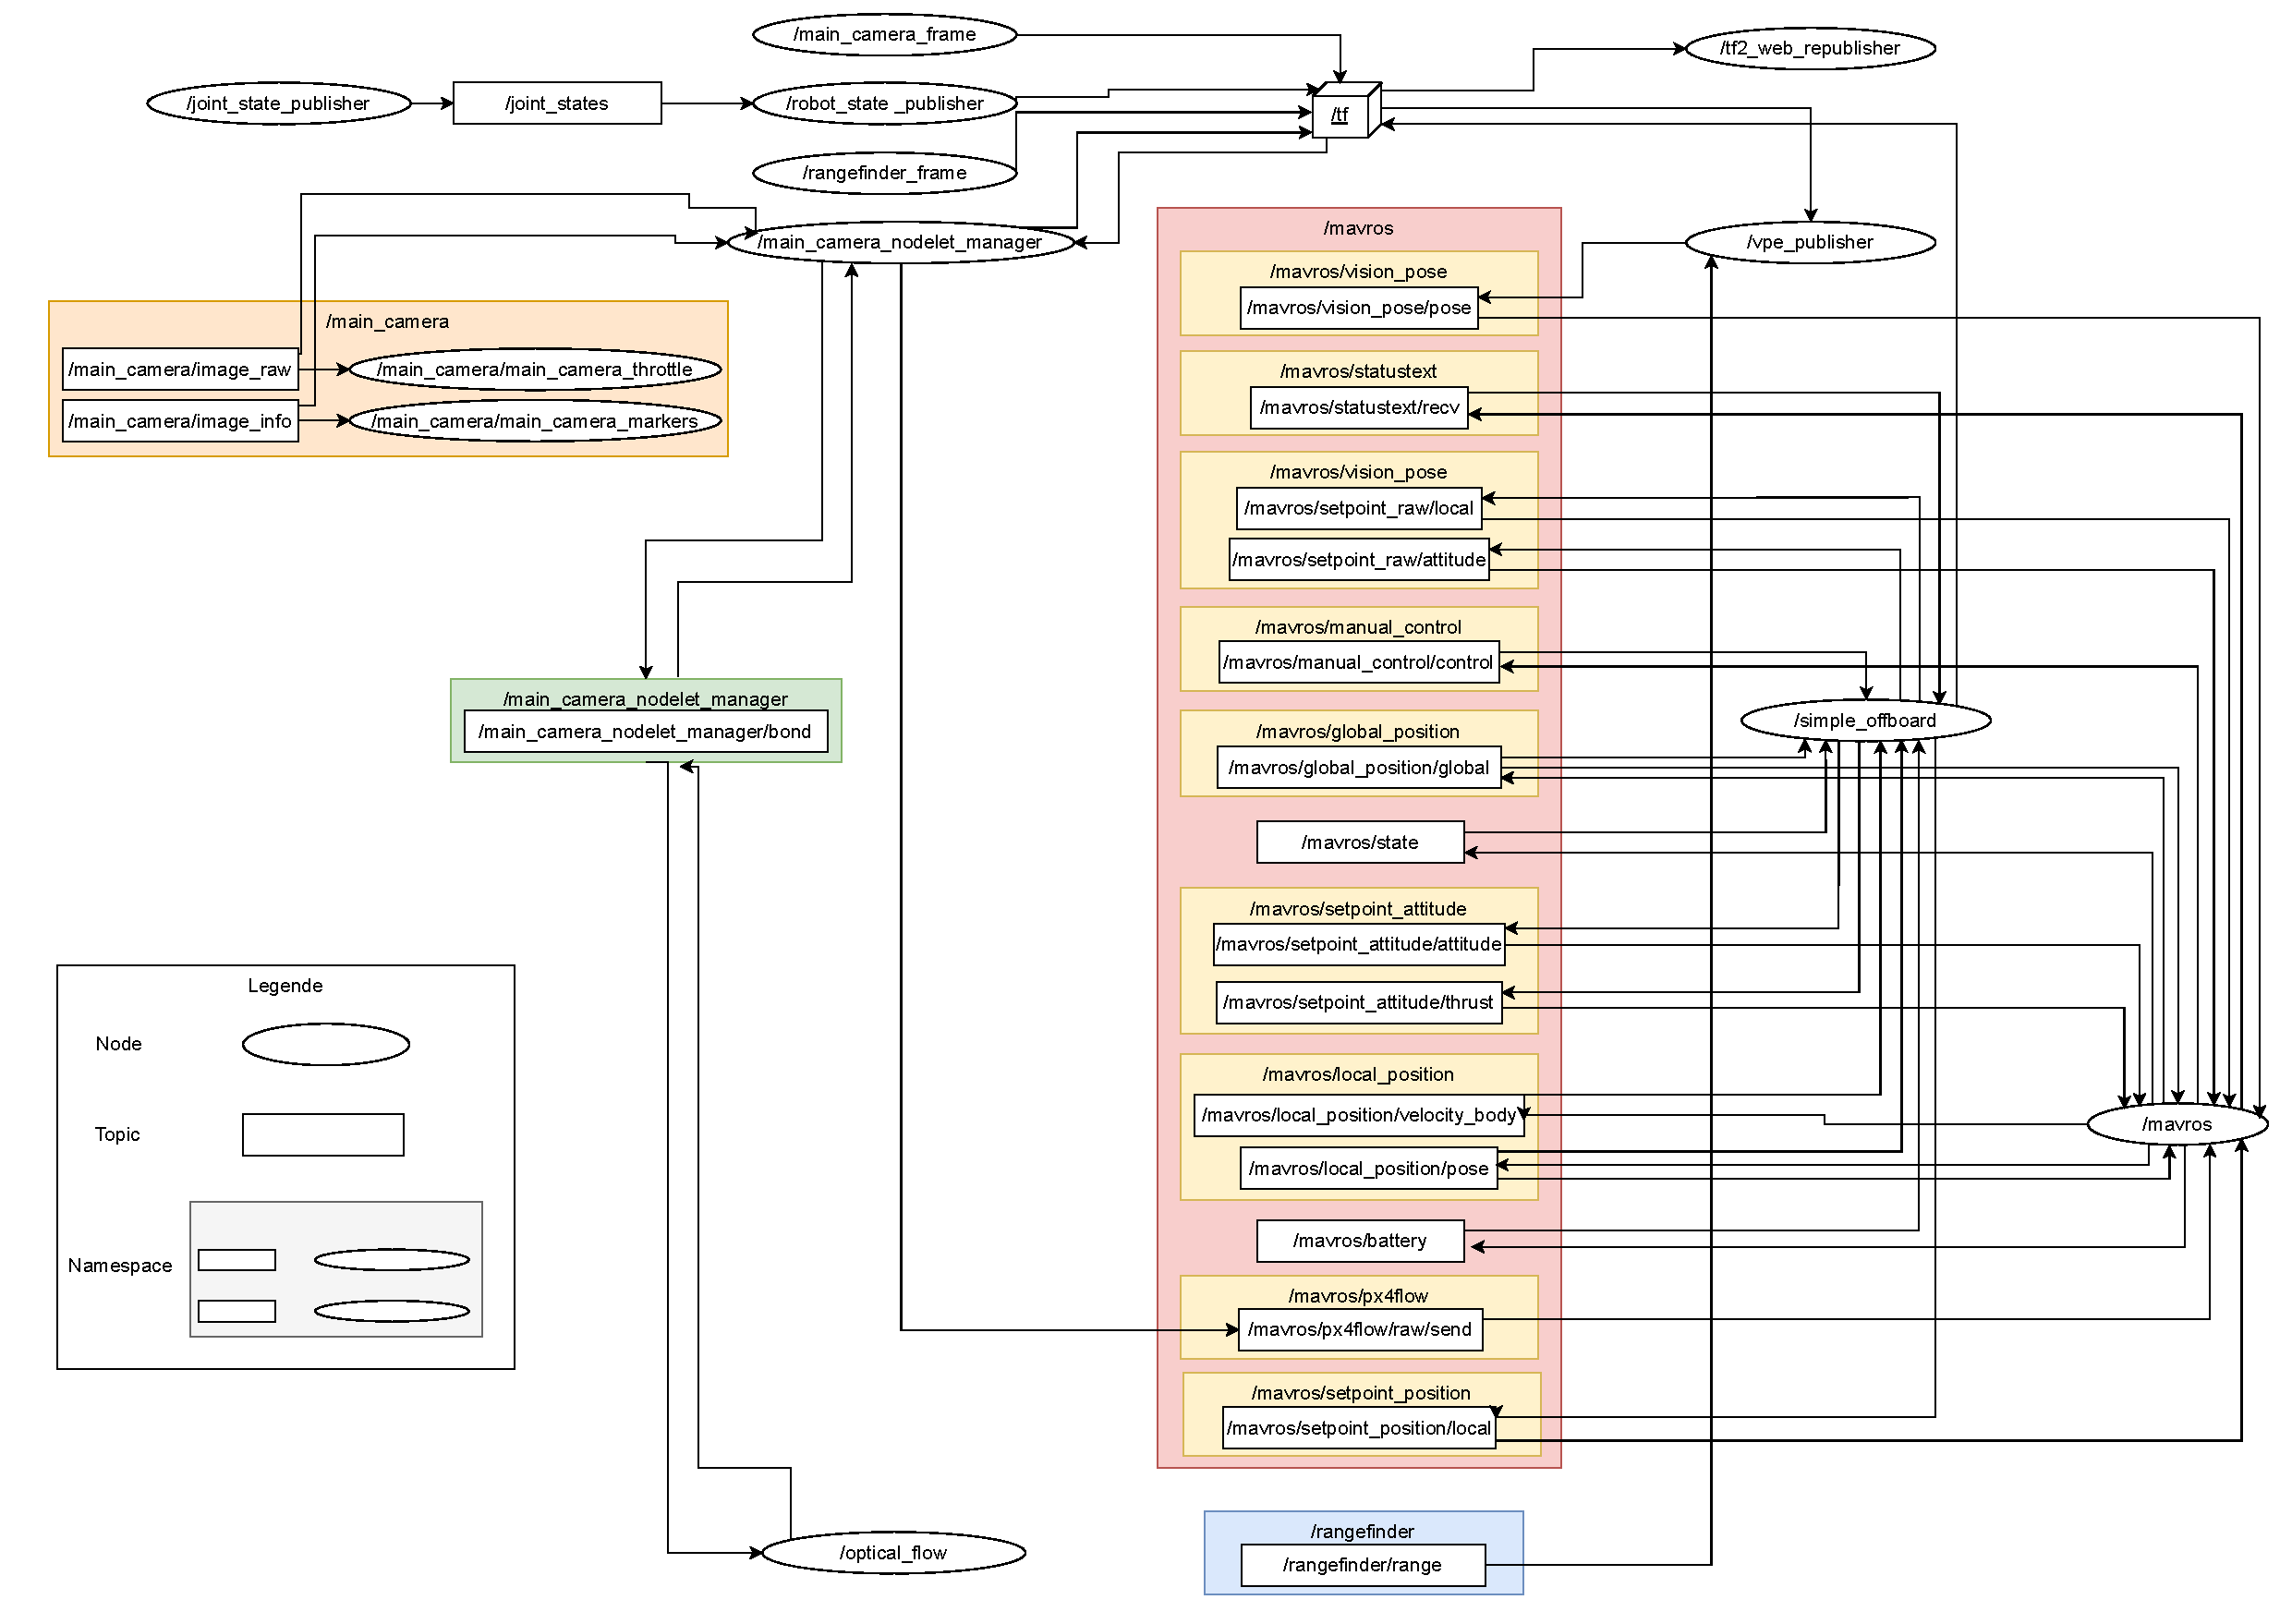
\includepdf[landscape=true]{images/graph_ros.pdf}
    %\caption[Übersicht ROS Nodes]{\label{img ros_nodes_graph} Übersicht ROS Nodes [eigene Darstellung]}
    \begin{landscape}
        \begin{figure}
            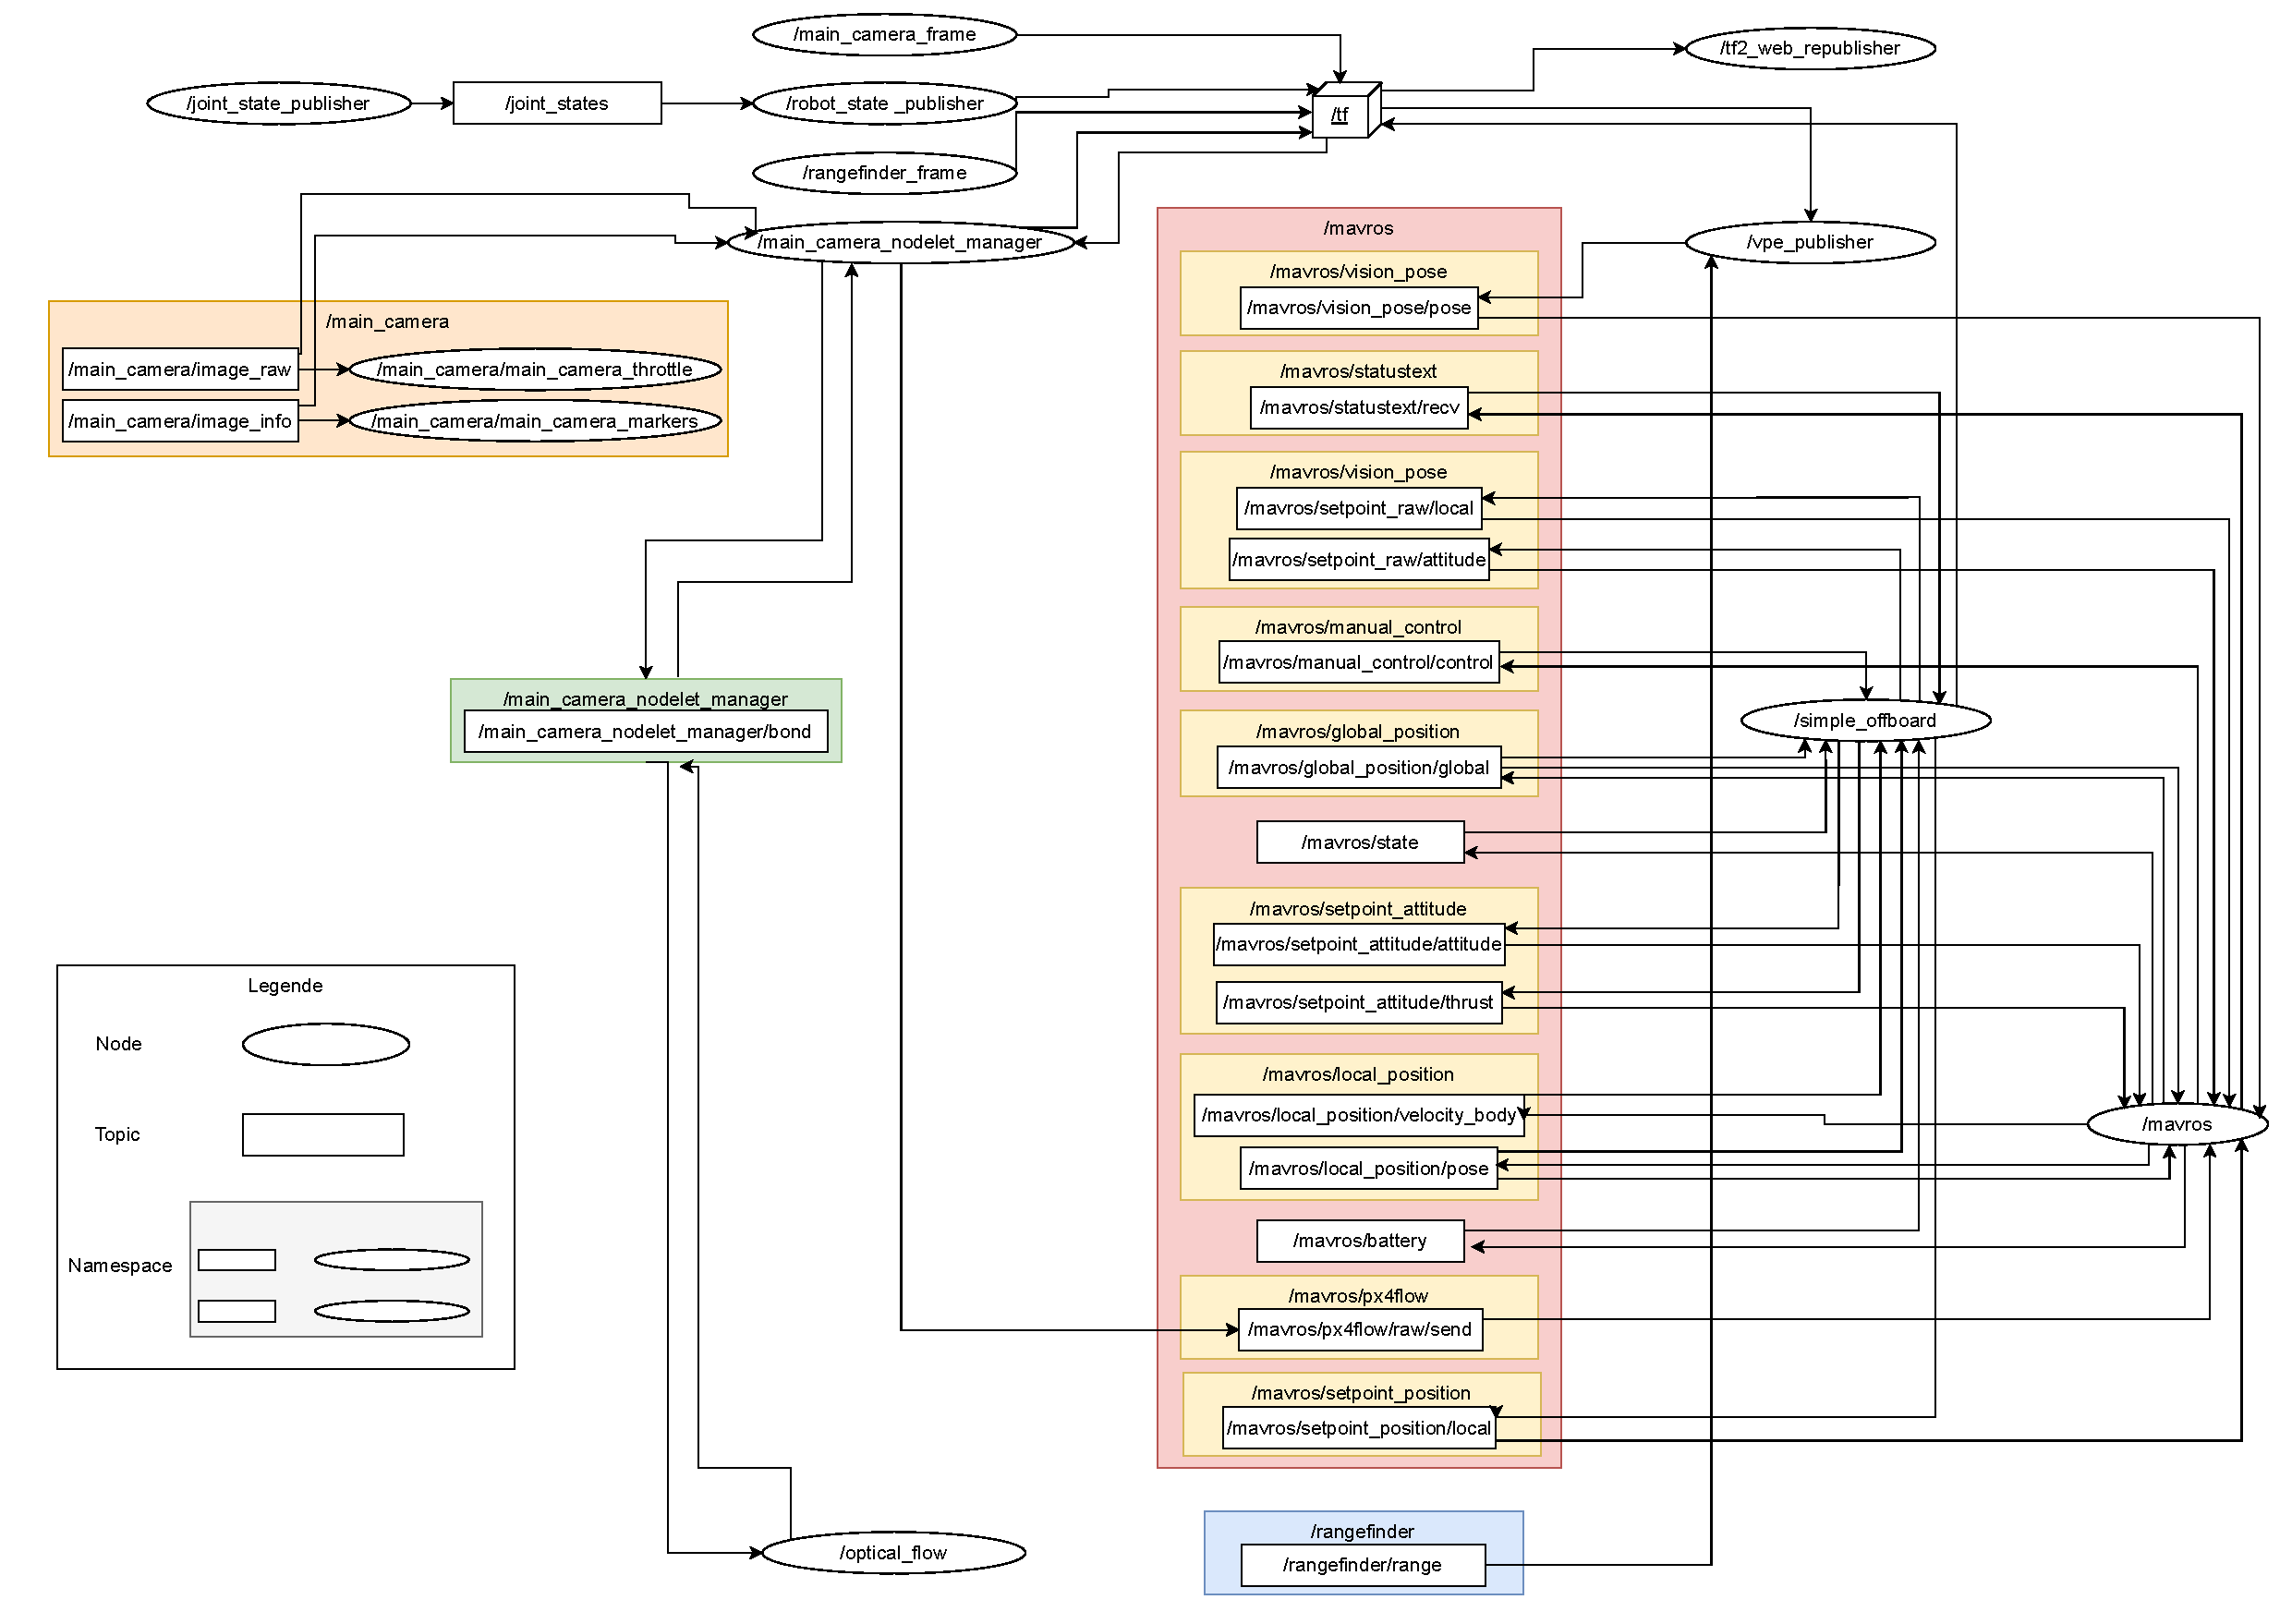
\includegraphics[width=\paperwidth,keepaspectratio]{images/graph_ros.pdf}
            \caption[Übersicht ROS Kommunikation]{\label{img ros_communication} Übersicht ROS Kommunikation [eigene Darstellung]}
        \end{figure}
    \end{landscape}

In der Abbildung \ref{img ros_communication} ist eine Übersicht der Kommunikation zwischen den verschiedenen Komponenten in \ac{ROS} zu sehen. \\
Hauptbestandteil sind hierbei vor allem die Nodes der Hauptkamera beziehungsweise der Azure Kinect sowie auch Mavros. \\
Mavros ist ein ROS-Paket, welches die Kommunikation zwischen dem Raspberry Pi und der Drohne mit Hilfe des MAVLink-Protokolls (siehe Kapitel \ref{mavlink}) ermöglicht. Es unterstützt dabei unter anderem den PX4 Flightstack, welcher in der Coex Clover Drohne vorhanden ist. Die Kommunikation kann hierbei wie bei MAVLink auch über \ac{USB} oder auch über Wifi stattfinden. \cite[vgl.][]{mavros}\\
Im nachfolgenden wird nun genauer auf die einzelnen Komponenten sowie den Ablauf der ROS Kommunikation (siehe \ref{img ros_communication}) eingegangen. \\

simple\_offboard: \\
simple\_offboard ermöglicht eine einfache Interaktion mit der Drohne. Das Modul hierzu vereinfacht das Programmieren von Skripten für autonome Flüge mit Drohnen mit Hilfe des Flugmodus Offboard. \cite[vgl.][]{simple_offboard}\\
% https://clover.coex.tech/en/simple_offboard.html

mavros: \\
Die Mavros Node ist für die Kommunikation zwischen dem Raspberry Pi und dem Flight Controller zuständig.\\
Hierfür gibt es viele verschiedene Topics, welche jeweils für den Austausch von unterschiedliche Informationen verantwortlich sind.\\
Diese Topics werden im Namespace "\textbackslash mavros" zusammengefasst, zu diesen zählen unter anderem:\\
\textbackslash mavros\textbackslash state: gibt den Status der Verbindung zwischen Raspberry Pi und Flightcontroller sowie den aktuellen Flugmodus an.\\
\textbackslash mavros\textbackslash battery: enthält verschiedene Parameter und Nachrichten zur Batterie. Hierzu zählen der aktuelle Ladezustand, die verbleibende Kapazität, die Spannung oder auch die geschätzte Restflugzeit der Drohne.\\
\textbackslash mavros\textbackslash local\_position\textbackslash pose: enthält die lokale Position sowie die aktuelle Orientierung der Drohne in einem Koordinatensystem.\\
\textbackslash mavros\textbackslash setpoint\_attitude\textbackslash attitude: enthält die Informationen zum Einstellen der Fluglage. \cite[vgl.][]{mavros}\\
% https://clover.coex.tech/en/mavros.html
 
main\_camera: \\
Von dem Azure Kinect ROS Treiber werden zwei Topics übergeben, diese sind: \\
"\textbackslash main\_camera\textbackslash image\_raw", über dieses Topic werden die Rohbilder der Kamera gesendet. Zudem noch "\textbackslash main\_camera\textbackslash image\_info", über welches die Kamerainformationen übertragen werden. \cite[vgl.][]{kinect_ros_driver}\\
\todo{author quelle?}
% https://github.com/microsoft/Azure_Kinect_ROS_Driver/blob/melodic/docs/usage.md

Der prinzipielle Ablauf bei der Kommunikation in Abbildung \ref{img ros_communication} wird von der mavros Node gestartet, denn diese bildet mit der Kommunikation zwischen ROS auf dem Raspberry Pi und dem PX4 des Flight Controllers die Grundlage. Zudem bietet der Einsatz der simple\_offboard Node die Möglichkeit zur Nutzung eigener Skripte, wodurch die Drohne autonom fliegen und navigieren kann. Diese beiden Nodes kommunizieren unter einander mit Hilfe der vielen verschiedenen Mavros-Nodes um Informationen und Parameter auszutauschen. Die simple\_offboard-Node kann zudem verschiedene Koordinatensysteme anfordern, welche von den Nodes aus dem main\_camera-Namespace kommen und mit Hilfe des \textbackslash tf-Topics transformiert werden. Diese Koordinatensysteme werden nun über die vpe\_publisher-Node an Mavros, sowie im weiteren Verlauf auch der simple\_offboard-Node übermittelt. Dadurch kann das Skript die Drohne anhand der Koordinaten navigieren und die Drohne dementsprechend zu der gewollten Position fliegen.
\todo{text überprüfen}
\todo{dopplungen entfernen} 

\section{Kalibrierung der COEX Drohne}

\section{Drohnen Autopilot}


\section{3D Modell}
Um die Drohne auch in der Simulation unter echten Bedingungen fliegen zu lassen, müssen die realen Gegebenheiten in die Simulation übertragen werden. Um dies zu bewerkstelligen, muss ein 3D-Modell der Räume erstellt werden, in welchen sich die Drohne bewegen soll.
    \subsection{3D Scan}

        \subsubsection{Microsoft HoloLens 2}
        Um ein 3D-Modell des Raumes mit der Microsoft HoloLens 2 zu erstellen, muss man die integrierte Mixed-Reality-Capture-Funktion der HoloLens 2 verwenden.
        
        Die Mixed-Reality-Capture-Funktion der HoloLens 2 ist eine integrierte Funktion, mit der Benutzer die Möglichkeit haben, die Hologramme, die von der HoloLens 2 dargestellt werden, in Echtzeit aufzuzeichnen und zu teilen. Diese Funktion ermöglicht es Benutzern, ihre Augenbewegungen und Handlungen in einer virtuellen Umgebung aufzuzeichnen, um sie mit anderen zu teilen oder für zukünftige Referenz oder Analyse zu speichern. Die Mixed-Reality-Capture-Funktion der HoloLens 2 kann auch für die Erstellung von Immersive-Mixed-Reality-Videoinhalten verwendet werden, indem sie es ermöglicht, virtuelle Hologramme in eine reale Umgebung zu integrieren. Dies kann für verschiedene Anwendungen wie zum Beispiel für die Erstellung von virtuellen Touren, für die Präsentation von Produkten oder für die Unterhaltungsindustrie eingesetzt werden.
        
        \todo{Erstellen des Modells beschreiben}

        Es ist wichtig zu beachten, dass die Qualität des erstellten 3D-Modells von verschiedenen Faktoren abhängt, wie z.B. der Beleuchtung im Raum und der Genauigkeit des Scans. Eine sorgfältige Vorbereitung des Raums und eine langsame, gründliche Durchführung des Scans können dazu beitragen, ein genaueres und detaillierteres 3D-Modell zu erstellen.
        \subsubsection{Azure Kinect \ac{DK}}

    \subsection{3D Modell Vorbereitung}

\section{Navigation}
% wie Navigation hätte umgesetzt werden können

% Navigation selbst nicht umgesetzt, u.a. auf Grund von Begrenzung Leistung Raspberry Pi




\section{Simulation}



